%----------------------------------------------------------------------------------------
%    PACKAGES AND THEMES
%----------------------------------------------------------------------------------------
\documentclass[aspectratio=169,xcolor=dvipsnames]{beamer}
\makeatletter
\def\input@path{{theme/}}
\makeatother
\usetheme{CleanEasy}
\usepackage[utf8]{inputenc}
\usepackage{lmodern}
\usepackage[T1]{fontenc}
% \usepackage[brazil]{babel}
\usepackage{fix-cm}
\usepackage{amsmath}
\usepackage{mathtools}
\usepackage{listings}
\usepackage{xcolor}
\usepackage{subcaption}
\usepackage{hyperref}
\usepackage{graphicx} % Allows including images
\usepackage{booktabs} % Allows the use of \toprule, \midrule and \bottomrule in tables
\usepackage{tikz}
\usetikzlibrary{positioning, shapes, arrows, calc, decorations.pathreplacing, arrows.meta, backgrounds, patterns, overlay-beamer-styles}
\usepackage{etoolbox}
\usepackage{animate}

\usepackage[backend=biber, style=ieee, sorting=nyt]{biblatex}
%\setlength{\bibitemsep}{0.8\baselineskip}
%\newcommand{\printbib}{%
%    \begin{spacing}{1}%
%    \printbibliography[heading={bibintoc}, title={References}]%
%    \end{spacing}%
%}

\addbibresource{reference.bib}


%----------------------------------------------------------------------------------------
%    LAYOUT CONFIGURATION
%----------------------------------------------------------------------------------------



% Configure code listings
\lstset{
  basicstyle=\ttfamily\small,
  keywordstyle=\color{blue},
  commentstyle=\color{green!60!black},
  stringstyle=\color{red},
  showstringspaces=false,
  breaklines=true,
  frame=single,
  rulecolor=\color{black},
  backgroundcolor=\color{black},
  numbers=left,
  numberstyle=\tiny\color{black},
  numbersep=5pt
}

%----------------------------------------------------------------------------------------
%    TITLE PAGE
%----------------------------------------------------------------------------------------


%---------------------------------------------

\title[A Data Driven Toggling Complementary Filtering Approach for Orientation Estimation]{
\vspace{-1.8cm}\\
A Data Driven Toggling Gain \\
Complementary Filtering Approach for \\
Orientation Estimation
}

\author[NDAG]{
\small 
\textbf{Network and Data Analysis Group} \\
Samnun Azfar - 200041130 \\  
Ramisa Zaman Audhi - 200041131 \\ 
Mir Md Inzamam - 200041240
}

\institute[VFU]{
    \vspace{0.2cm} \\
    \begin{tabular}{c c}
        \textbf{Supervised by} & \textbf{Co-supervised by} \\
        Abu Raihan Mostofa Kamal & Mohammad Ishrak Abedin \\
        Professor & Lecturer \\  
        Department of CSE & Department of CSE \\
        Islamic University of Technology & Islamic University of Technology
    \end{tabular}
}

\date{April 29, 2025} 

\titlegraphic{
  \begin{tikzpicture}[remember picture, overlay]
    \node[anchor=north east, xshift=-0.8cm, yshift=-0.3cm] at (current page.north east) {
      \includegraphics[height=1.5cm]{logos/iutlogo.jpeg}
    };
  \end{tikzpicture}
}


%----------------------------------------------------------------------------------------


\begin{document}

\begin{frame}[plain]
  \titlepage
\end{frame}

% \begin{frame}[plain]{Contents}
%   \tableofcontents
% \end{frame}

\section{Introduction}


\begin{frame}{Orientation Algorithms in Real World Applications}
\tiny
\begin{columns}[T]
  % Top row: two images, fixed height
  \column{0.48\textwidth}
    \centering
    \includegraphics[height=2.5cm]{logos/a-Inertial-measurement-unit-IMU-placed-over-the-head-mounted-display-HMD-b.png} \\[0.3em]
    \href{https://www.mdpi.com/1424-8220/23/6/3077}{VR Head‐mount}
  \column{0.48\textwidth}
    \centering
    \includegraphics[height=2.5cm]{logos/smartphone.jpg} \\[0.3em]
    \href{https://www.mdpi.com/1424-8220/24/15/4769}{Smartphone orientation}
\end{columns}

\vspace{0.6em}

% Bottom row: one image
\begin{center}
  \includegraphics[height=3.5cm]{logos/autonomous.jpg} \\[0.3em]
  \href{https://www.sbg-systems.com/vehicles/self-driving-cars/}{Autonomous vehicles}
\end{center}
\end{frame}



\begin{frame}{IMUs and MARG Sensors}
\hfill
\begin{figure}
    \centering
    \includegraphics[width=0.55\linewidth]{logos/IMU-Applications-EN-768x671.png}
    \caption{\href{https://atadiat.com/en/e-towards-understanding-imu-basics-of-accelerometer-and-gyroscope-sensors/}{IMU and MARG sensors applications}}
    \label{fig:imuapp}
\end{figure}
\hfill
\end{frame}


\begin{frame}{Sensor Fusion Concept}
\begin{itemize}
  \item Individual sensors have complementary strengths: 
    - \textbf{gyroscopes} measure rotation but \textcolor{red}{drift over time}, \textbf{accelerometers} measure tilt via gravity but are \textcolor{red}{noisy during movement}, \textbf{magnetometers} give heading but are \textcolor{red}{disturbed by local fields}.
  \item Sensor fusion algorithms (e.g., Kalman\cite{EKF}\cite{doubleEKF}\cite{quatEKF} or complementary filters\cite{compfilter}) combine these readings to obtain a stable orientation estimate. By using multiple sensors, we can \textcolor{blue}{“reduce orientation drift introduced through the gyroscope measurements”} using gravity and magnetic references.
\end{itemize}
\begin{block}{Goal}
    The goal is to filter out noise and biases: high-frequency noise from accelerometers is smoothed, while low-frequency gyro drift is corrected by accelerometer/magnetometer data, yielding a robust attitude estimate.
\end{block}
\end{frame}

\begin{frame}{Complementary Filter (CF) Approach}
\begin{itemize}
  \item The complementary filter \textbf{fuses gyro and accelerometer data} by applying a \textcolor{blue}{high-pass filter to the \textbf{gyro} (tracking quick changes)} and a \textcolor{blue}{low-pass filter to the \textbf{accelerometer} (tracking slow changes)}\cite{compfilter}.
\end{itemize}
\begin{block}{General Equation of the weighted sum}
    \textbf{$\theta(t)=(1 - \alpha)\,(\text{gyro-integrated angle}) + \alpha\,(\text{accel-derived angle})$}
\end{block}
\begin{itemize}
  \item The blending weight \textbf{$\alpha$} (between 0 and 1) is tuned based on sensor characteristics. 
  \item This yields the \textbf{“best of both worlds”}: the gyro provides a smooth angle during motion, and the accelerometer corrects long-term drift. Properly tuned, the CF can yield orientation with low noise and low.
\end{itemize}
\end{frame}

\begin{frame}{Complementary Filter: Pros and Cons}
\begin{columns}[T,onlytextwidth]
  % Left: Advantages
  \begin{column}{0.48\textwidth}
    \begin{block}{\textbf{Advantages}}
      \begin{itemize}
        \item Very simple and efficient to implement on micro-controllers.
        \item Requires minimal computation.
        \item Effectively reduces random noise (accelerometer) and drift (gyroscope)\cite{valentiCF2015}.
      \end{itemize}
    \end{block}
  \end{column}
  % Right: Disadvantages
  \begin{column}{0.48\textwidth}
    \begin{block}{\textbf{Disadvantages}}
      \begin{itemize}
        \item Fixed filter gains cannot adapt to changing dynamics or sensor conditions.
        \item Gyroscope biases over time introduce drift if not perfectly zeroed.
        \item Assumes a stable magnetic reference—magnetic disturbances cause yaw drift.
      \end{itemize}
    \end{block}
  \end{column}
\end{columns}

\vspace{0.5em}
In summary, CF is computationally light and effective for many scenarios but can struggle during aggressive motion or magnetic interference, motivating adaptive extensions.
\end{frame}


\section{Uses and Applications}

\begin{frame}{Consequences of Poor Orientation Estimation}
\begin{itemize}
  \item In \textcolor{blue}{\textbf{VR/AR}}, \textbf{incorrect orientation} causes virtual objects to \textbf{lag or shift unexpectedly}, leading to \textcolor{red}{user disorientation or motion sickness}. The “reality” no longer matches the user’s motions.
  \item In \textcolor{blue}{\textbf{navigation (drones, aircraft, robotics)}}, \textbf{bad attitude estimates} can cause \textcolor{red}{control errors or crashes}. For example, a drone in strong magnetic interference may misread its yaw and slowly rotate off course.
  \item \textcolor{blue}{\textbf{Inertial systems}} are immune to jamming (no external signals needed), but they rely on \textbf{sensor accuracy}. If magnetic disturbances occur, a MARG system \textcolor{red}{“will over time result in a drift in the heading estimate”}.
\end{itemize}
Therefore, improving orientation accuracy is critical for safety and user experience.
\end{frame}

\begin{frame}{Data-Driven and Machine Learning Methods}
\centering

\begin{itemize}
  \item Modern approaches use \textbf{data analysis and machine learning} to enhance orientation filters. For example, auxiliary sensor data (like eye tracking) can be fused to detect motion phases and correct drift.
  \item Machine learning can learn \textbf{complex biases or map raw sensor patterns to orientation}, effectively “calibrating” IMUs from data. Recent studies show ML-tuned filters outperform fixed filters in sports and motion tracking.
  \item This aligns with the data science paradigm: extracting knowledge and patterns from data to make better. By analyzing large IMU datasets, ML models can improve orientation estimates beyond classic CF assumptions.
\end{itemize}
\begin{exampleblock}{Best of both worlds?}
    Combining \textbf{traditional filters} with \textbf{data-driven tuning} offers more adaptive, accurate orientation estimation \cite{vertzberger2022adaptive}.
\end{exampleblock}
\end{frame}

\section{Literature Review}

\begin{frame}{Literature Review (Paper 1)}

\textbf{Adaptive Attitude Estimation Using a Hybrid Model-Learning Approach (2022)} \hfill \textcolor{blue}{\cite{vertzberger2022adaptive}}\\
\textbf{Authors:} Eran Vertzberger, Itzik Klein \\
\textbf{Journal:} IEEE Transactions on Instrumentation and Measurement

\vspace{1em}
\scriptsize
\begin{columns}
    \column{0.5\textwidth}
    \textbf{Overview:}\\
    Demonstrates a \textbf{hybrid adaptive complementary filter} that learns axis-specific accelerometer weights via neural networks. Quaternion gyro data is integrated and a complementary update is applied in each axis whose weight is predicted by a small neural network based on estimated linear accelerations. 

    \vspace{0.5em}
    \textbf{Evaluation:}
    \begin{itemize}
        \item Smartphone IMU dataset (60 two‑minute sequences of walking activities in pocket, hand, etc., with VI‑SLAM ground truth)
    \end{itemize}
    
    \textbf{Benchmark:}
    \begin{itemize}
        \item Fixed-gain filters (Mahony\textcolor{blue}{\cite{mahony2008nonlinear}}, Madgwick\textcolor{blue}{\cite{madgwick2011estimation}})
    \end{itemize}

    \column{0.5\textwidth}
    \textbf{Contributions:}
    \begin{itemize}
        \item Learned filter (DAE) yielded the lowest roll/pitch errors (10–37\% better than classic filters).
        \item Adapts to dynamic motion via data-driven weight tuning.
        \item Outperforms fixed gains under varying conditions.
    \end{itemize}

    \vspace{0.5em}
    \textbf{Disadvantages:}
    \begin{itemize}
        \item Requires labeled training data and offline learning.
        \item Neural nets add complexity.
        \item Yaw is not addressed (no magnetometer fusion).
    \end{itemize}
\end{columns}

\end{frame}

\begin{frame}{Literature Review (Paper 2)}

\textbf{A Robust Complementary Filter Approach for Attitude Estimation of Unmanned Aerial Vehicles using AHRS (2019) \hfill \textcolor{blue}{\cite{CEAS-GNC-2019-036}}}\\
\textbf{Authors: }Johann Meyer, Kreelan Padayachee, Benjamin A. Broughton \\
\textbf{Conference: }CEAS EuroGNC 2019

\vspace{1em}
\scriptsize
\begin{columns}
    \column{0.5\textwidth}
    \textbf{Overview:}\\
     Explicitly detects when accelerometers are unreliable based on “steadiness” measure (using a low‑pass on the accel magnitude) to decide if the vehicle is in steady flight. When unsteady, the filter relies on gyro propagation only; when steady, normal fusion occurs. A Gaussian random-walk model for gyro bias is implemented that rejectsimprobable bias drifts during maneuvers. 
    \vspace{0.5em}
    \textbf{Evaluation:}
    \begin{itemize}
        \item Monte Carlo simulations (maneuvering UAV trajectories)
    \end{itemize}

    \column{0.5\textwidth}
    \textbf{Contributions:}
    \begin{itemize}
        \item Monte Carlo simulations show their filter tracks roll dynamics more accurately than standard CFs\textcolor{blue}{\cite{compfilter}}. 
        \item Simple gating logic avoids gross errors from accelerometer disturbances. 
        \item Robust gyro bias handling.
    \end{itemize}

    \vspace{0.5em}
    \textbf{Disadvantages:}
    \begin{itemize}
        \item Effectively disables accelerometer fusion during dynamics (so short-term drift may grow). 
        \item Requires tuning of “steadiness” thresholds. 
        \item Only tested in simulations.
    \end{itemize}
\end{columns}

\end{frame}

\begin{frame}{Literature Review (Paper 3)}

\textbf{Adaptive Complementary Filtering Algorithm for IMU Based on MEMS (2020)} \hfill \textcolor{blue}{\cite{wang2020mems}}\\
\textbf{Authors:} Zhang Zhe, Wang Jian-bin, Song Bo, Tong Guo-feng \\
\textbf{Conference:} 2020 Chinese Control and Decision Conference, CCDC, IEEE

\vspace{1em}
\scriptsize
\begin{columns}
    \column{0.5\textwidth}
    \textbf{Overview:}\\
    An \textbf{adaptive sparse-interpolation CF (ASICF)} has been proposed for MEMS IMUs. A quaternion-based complementary filter is used to fuse gyro and accel, but an adaptive data-skip mechanism is added: the filter monitors consecutive accelerometer samples, assesses the “trustworthiness” of the accel (via its variation), and if the data are too noisy or dynamic, it performs an interpolation step rather than using the raw sample (downsampling).

    \vspace{0.5em}
    \textbf{Evaluation:}
    \begin{itemize}
        \item Multiple datasets (drone, car, human motion)
    \end{itemize}
    
    \textbf{Benchmark:}
    \begin{itemize}
        \item Fixed-gain filters (Mahony\textcolor{blue}{\cite{mahony2008nonlinear}}, Madgwick\textcolor{blue}{\cite{madgwick2011estimation}}), Valenti CF\textcolor{blue}{\cite{valentiCF2015}}
    \end{itemize}

    \column{0.5\textwidth}
    \textbf{Contributions:}
    \begin{itemize}
        \item  Reported significantly lower attitude errors under large disturbances (e.g. 20\% smaller error than the Valenti CF \textcolor{blue}{\cite{valentiCF2015}}). 
        \item Can handle sudden motions by effectively smoothing or skipping bad accelerometer readings.
        \item Retains quaternion CF structure.
    \end{itemize}

    \vspace{0.5em}
    \textbf{Disadvantages:}
    \begin{itemize}
        \item Performance depends on correctly detecting outliers.
        \item May introduce lagging when interpolating
    \end{itemize}
\end{columns}

\end{frame}

\begin{frame}{Literature Review (Paper 4)}
    
\textbf{A Variable Gain Complementary Filtering Fusion Algorithm Based on Distributed Inertial Network and Flush Air Data Sensing (2023)} \hfill \textcolor{blue}{\cite{shao2023variablegainflushsesnsing}}\\
\textbf{Authors:} Weiguang Shao, Jianwen Zang, Jin Zhao and Kai Liu\\
\textbf{Journal:} Applied Sciences (ISSN 2076-3417) 2023, MDPI

\vspace{1em}
\scriptsize
\begin{columns}
    \column{0.5\textwidth}
    \textbf{Overview:}\\
     A \textbf{variable-gain CF for aircraft angle-of-attack estimation} is introduced which uses a distributed IMU network plus flush-air sensors. A flight-phase-dependent blending factor is derived: the filter coefficient (analogous to $\alpha$) which is allowed to vary with the change rate of the angle-of-attack, placing more weight on inertial data at high dynamics. 

    \column{0.5\textwidth}
    \textbf{Contributions:}
    \begin{itemize}
        \item  Simulation results for a high-speed UAV show this VGCF yields significantly smaller AoA error than a constant-gain INS+FADS filter (approximately 0.0058° vs 0.0017° RMSE, i.e. >2× improvement)
        \item Adapts filtering to flight conditions, mitigating delay in air-data measurements
    \end{itemize}

    \vspace{0.5em}
    \textbf{Disadvantages:}
    \begin{itemize}
        \item Heavily domain-specific (flush-air data, aerodynamic model). 
        \item Complexity of inertial network fusion. 
    \end{itemize}
\end{columns}

\end{frame}

\begin{frame}{Literature Review (Paper 5)}

\textbf{Denoising IMU Gyroscopes With Deep Learning for Open-Loop Attitude Estimation (2020)} \hfill \textcolor{blue}{\cite{brossard2020openloopCNN}}\\
\textbf{Authors:} Martin Brossard, Silvère Bonnabel, Axel Barrau \\
\textbf{Journal:} IEEE Robotics and Automation Letters (Volume: 5, Issue: 3, July 2020)

\vspace{1em}
\scriptsize
\begin{columns}
    \column{0.5\textwidth}
    \textbf{Overview:}\\
    A \textbf{deep convolutional network} to denoise IMU gyroscopes for open-loop attitude estimation is introduced, where a CNN (with dilated convolutions) is trained on ground-truth data so that it outputs corrected gyro increments. The orientation is then obtained by simply integrating these denoised increments in dead-reckoning. Their loss is carefully designed for angular increments, and no RNNs are used (making inference fast). 

    \vspace{0.5em}
    \textbf{Evaluation:}
    \begin{itemize}
        \item EuRoC and TUM-VI Datasets
    \end{itemize}

    \column{0.5\textwidth}
    \textbf{Contributions:}
    \begin{itemize}
        \item  Outperforms state‑of‑the‑art methods and even beats top visual–inertial odometry algorithms in attitude accuracy. 
        \item End-to-end learned correction captures complex noise/scale drift. 
        \item No vision needed yet achieves very low drift.
    \end{itemize}

    \vspace{0.5em}
    \textbf{Disadvantages:}
    \begin{itemize}
        \item Requires large ground-truth datasets for training design is more complex.
        \item Open-loop mode still drifts (albeit slower).
        \item Network complexity. 
    \end{itemize}
\end{columns}

\end{frame}

\begin{frame}{Literature Review (Paper 6)}

\textbf{Generalizable End-to-End Deep Learning Frameworks for Real-Time Attitude Estimation Using 6DoF Inertial Measurement Units (2023)} \hfill \textcolor{blue}{\cite{golroudbari2023cnn6DOF}}\\
\textbf{Authors:} Arman Asgharpoor Golroudbari, Mohammad Hossein Sabour \\
\textbf{Journal:} Measurements (Volume 217, 113105) Elsevier

\vspace{1em}
\scriptsize
\begin{columns}
    \column{0.5\textwidth}
    \textbf{Overview:}\\
    An \textbf{end-to-end neural IMU attitude estimator} is proposed. Two deep models (CNN+BiLSTM+FC) are trained to directly map 6-DOF IMU sequences to quaternions. Training uses seven public datasets (120+ hours of motion). Their models generalize across different motions, sampling rates and disturbances, and they report higher accuracy than prior methods. 

    \vspace{0.5em}
    \textbf{Evaluation:}
    \begin{itemize}
        \item Seven public datasets including EuRoC and TUM-VI
    \end{itemize}

    \column{0.5\textwidth}
    \textbf{Contributions:}
    \begin{itemize}
        \item Leverages temporal convolution and recurrent units for rich modeling.
        \item Tested on massive diverse data 
    \end{itemize}

    \vspace{0.5em}
    \textbf{Disadvantages:}
    \begin{itemize}
        \item Heavy models requiring long training. 
        \item \textbf{“Black box”}, so no physical insight. 
        \item Relies on availability of similar data during training.  
    \end{itemize}
\end{columns}

\end{frame}

% Slide 1
\begin{frame}{Gaps and Opportunities (1/3)}
\scriptsize
\begin{columns}[T]
    \begin{column}{0.48\textwidth}
    \begin{block}{{\textbf{Lack of Real-Time Adaptivity}}}
    \begin{itemize}
        \item Static parameters cannot adapt to dynamic changes \cite{madgwick2011estimation}\cite{compfilter}\cite{rosario2016smartphonequat}
        \item Unexpected accelerations degrade accuracy \cite{vandijk2021mlreview}
    \end{itemize}
    \end{block}
    \end{column}
    
    \begin{column}{0.48\textwidth}
    \begin{exampleblock}{{\textbf{Solution: Adaptive Learning}}}
    \begin{itemize}
        \item Dual-XGBoost adjusts fusion weights online from incoming IMU data.
        \item Responds dynamically to abrupt motions or disturbances.
    \end{itemize}
    \end{exampleblock}
    \end{column}
\end{columns}

\vspace{0.8em}

\begin{columns}[T]
    \begin{column}{0.48\textwidth}
    \begin{block}{{\textbf{Lack of Explicit Noise Prediction}}}
    \begin{itemize}
        \item Assumes constant noise \cite{EKF}\cite{quatEKF}\cite{doubleEKF} can't predict sensor drift \cite{damagatla2024xgboostnoiseekf}.
        \item Can't handle temperature-induced or vibration noise changes\cite{damagatla2024xgboostnoiseekf}.
    \end{itemize}
    \end{block}
    \end{column}
    
    \begin{column}{0.48\textwidth}
    \begin{exampleblock}{{\textbf{Solution: Predictive Noise Modeling}}}
    \begin{itemize}
        \item XGBoost predicts gyro bias/variance from real-time sensor data.
        \item Learns time-varying noise models to maintain estimation accuracy.
    \end{itemize}
    \end{exampleblock}
    \end{column}
\end{columns}
\end{frame}

% Slide 2
\begin{frame}{Gaps and Opportunities (2/3)}
\scriptsize
\begin{columns}[T]
    \begin{column}{0.48\textwidth}
    \begin{block}{{\textbf{Over-Reliance on Fixed Gains}}}
    \begin{itemize}
        \item Fixed gains cause large estimation errors in dynamic motions \cite{vandijk2021mlreview}\cite{madgwick2011estimation}
        \item Can't balance between under-correction and over-correction\cite{shao2023variablegainflushsesnsing}\cite{EKF}
    \end{itemize}
    \end{block}
    \end{column}
    
    \begin{column}{0.48\textwidth}
    \begin{exampleblock}{{\textbf{Solution: Dynamic Gain Tuning}}}
    \begin{itemize}
        \item XGBoost adaptively infers fusion weights from current IMU readings.
        \item Eliminates need for manual gain tuning.
    \end{itemize}
    \end{exampleblock}
    \end{column}
\end{columns}

\vspace{0.8em}

\begin{columns}[T]
    \begin{column}{0.48\textwidth}
    \begin{block}{{\textbf{Challenge: Heavy Computational Burden}}}
    \begin{itemize}
        \item DNNs\cite{golroudbari2023cnn6DOF}\cite{CEAS-GNC-2019-036}\cite{brossard2020openloopCNN} and advanced EKFs\cite{EKF}\cite{doubleEKF} are too heavy for real-time embedded systems.
        \item Require GPUs or powerful processors\cite{chen2024dlsurvey}.
    \end{itemize}
    \end{block}
    \end{column}
    
    \begin{column}{0.48\textwidth}
    \begin{exampleblock}{{\textbf{Solution: Lightweight Inference}}}
    \begin{itemize}
        \item XGBoost is efficient at runtime: fast tree traversal, no heavy matrix ops.
        \item Suitable for real-time operation on micro-controllers.
    \end{itemize}
    \end{exampleblock}
    \end{column}
\end{columns}
\end{frame}

% Slide 3
\begin{frame}{Gaps and Opportunities (3/3)}
\scriptsize
\begin{columns}[T]
    \begin{column}{0.48\textwidth}
    \begin{block}{{\textbf{Loss of Interpretability}}}
    \begin{itemize}
        \item Deep models\cite{golroudbari2023cnn6DOF}\cite{CEAS-GNC-2019-036}\cite{brossard2020openloopCNN} are black-box; internal logic is opaque.
        \item Lack of physical insight makes debugging difficult \cite{chen2024dlsurvey}.
    \end{itemize}
    \end{block}
    \end{column}
    
    \begin{column}{0.48\textwidth}
    \begin{exampleblock}{{\textbf{Solution: Transparent Design}}}
    \begin{itemize}
        \item XGBoost trees are interpretable: splits and feature importance visible.
        \item Fusion logic explicitly maintains ties to physics.
    \end{itemize}
    \end{exampleblock}
    \end{column}
\end{columns}
\end{frame}
\section{Proposed Solution}

\begin{frame}{Proposed Modified Complementary Filter}
\scriptsize
\begin{columns}[T]
  % Noise Prediction & Removal
  \begin{column}{0.48\textwidth}
    \begin{block}{{Noise Prediction \& Removal} \cite{brossard2020openloopCNN}}
      \begin{itemize}
        \item Input raw sensor (acc, mag, gyro) columns: 
          $a_i=(a_{ix},a_{iy},a_{iz})$, 
          $m_i=(m_{ix},m_{iy},m_{iz})$, 
          $g_i=(g_{ix},g_{iy},g_{iz})$.
        \item Trained regressor predicts noise components $\eta_a,\eta_m$.
        \item Denoised vectors:
          \[
            a_i = a_i - \eta_a,\quad
            m_i = m_i - \eta_m 
          \]
          \[
            a_{\textit{pred}} = R_g*a_{(i-1)pred}(1-\alpha) + \alpha*a_i
          \]
          \[
            m_{\textit{pred}} = R_g*m_{(i-1)pred}(1-\alpha) + \alpha*m_i
          \]
        \item In the above equations $R_{g}$ is the quaternion or rotation matrix \cite{black1964passive}\cite{cariow2016hardware}.
      \end{itemize}
    \end{block}
  \end{column}
  % Movement Prediction & Alpha Toggling
  \begin{column}{0.48\textwidth}
    \begin{block}{{Movement Prediction \& $\alpha$ Toggling} \cite{vertzberger2022adaptive}}
      \begin{itemize}
        \item Toggling Engine analyzes $g_i$ (gyro) patterns to classify motion state.
        \item Generates adaptive gain $\alpha$ based on predicted movement (static vs.\ dynamic).
        \item Compute gyro‐based update:
        \[
          R_g = \exp\bigl(\Omega_{\times}(g_i)\,\delta t\bigr)
        \]
        where $\Omega_{\times}$ is the skew‐symmetric operator \cite{zhao2016time}.
        \item Final CF fusion in \autoref{fig:twinboost}:
        \[
          R = (1-\alpha)\,R_g \;+\;\alpha\,R_{am}.
        \]
      \end{itemize}
    \end{block}
  \end{column}
\end{columns}
\end{frame}



\begin{frame}{Proposed Modified Complementary Filter}
\begin{figure}
    \centering
    \includegraphics[width=1\linewidth]{logos/workflownew.png}
    \caption{Toggling Engine: Modified Filter Diagram with Noise Prediction and Movement Prediction}
    \label{fig:twinboost}
\end{figure}
\end{frame}

\begin{frame}{XGBoost Ensemble}
\begin{figure}
    \centering
    \includegraphics[width=0.6\linewidth]{logos/ensemble.png}
    \label{fig:twinboost}
    \caption{Prediction of One component of noise through an Ensemble model(XGB in our case)}
\end{figure}
\end{frame}


% Slide 1: Dataset Overview
\begin{frame}{Dataset Overview: BROAD}
\begin{itemize}
  \item \textbf{Berlin Robust Orientation Estimation Assessment Dataset (BROAD)} \cite{BROAD}
  \item \textbf{Trials:} 39 recordings of predefined motions
  \item \textbf{Sampling:}
    \begin{itemize}
      \item OptiTrack ground truth: position {opt\_pos} \& orientation {opt\_quat} at 120Hz
      \item IMU MARG data: accelerometer, gyroscope, magnetometer at \SI{286}{Hz}
      \item Boolean movement flag per timestamp
    \end{itemize}
  \item \textbf{Hardware:}
    \begin{itemize}
      \item Custom 3D-printed mount with myon aktos-t 9-axis IMU
      \item Optical markers for tracking by OptiTrack OMC system
    \end{itemize}
  \item \textbf{Motion types:} undisturbed (rotation, translation, combined; slow/fast) and disturbed (tapping, vibration, magnets, office, mixed)
  \item Detailed protocol in the BROAD paper: \url{https://www.mdpi.com/2306-5729/6/7/72}
\end{itemize}
\end{frame}

% Slide 2: Trial Categories & Figures
\begin{frame}{Dataset Details: Categories \& Hardware}
\scriptsize
\begin{columns}[T]
  % Left: table
  \begin{column}{0.48\textwidth}
      \begin{tabular}{|p{0.30\textwidth}|p{0.12\textwidth}|p{0.10\textwidth}|}
        \hline
        \textbf{Motion Type} & \textbf{Speed} & \textbf{Indices} \\ \hline
        \multicolumn{3}{|l|}{\textbf{Undisturbed}} \\ \hline
        Rotation    & Slow & 01–05 \\ 
        Rotation    & Fast & 06–09 \\
        Translation & Slow & 10–14 \\
        Translation & Fast & 15–18 \\
        Combined    & Slow & 19–20 \\
        Combined    & Fast & 21–23 \\ \hline
        \multicolumn{3}{|l|}{\textbf{Disturbed (Medium Speed)}} \\ \hline
        Tapping               & — & 24–25 \\
        Vibrating Smartphone  & — & 26–27 \\
        Stationary Magnet     & — & 28–31 \\
        Attached Magnet (1–5) & — & 32–36 \\
        Office Environment    & — & 37–38 \\
        Mixed                 & — & 39     \\ \hline
      \end{tabular}
    
  \end{column}

  % Right: figures
  \begin{column}{0.5\textwidth}
    \begin{figure}
      \centering
      \begin{subfigure}[t]{\columnwidth}
        \includegraphics[width=0.5\linewidth]{logos/dataset.png}
        \caption{Dataset columns overview}
        \label{fig:datase}
      \end{subfigure}
      \vspace{0.5em}
      \begin{subfigure}[t]{\columnwidth}
        \includegraphics[width=0.5\linewidth]{logos/imu_hardware_mount.png}
        \caption{3D-printed mount with IMU (OptiTrack markers)}
        \label{fig:IMUhardware}
      \end{subfigure}
    \end{figure}
  \end{column}
\end{columns}
\end{frame}

\section{Experimental Setup}

\begin{frame}{Training to Predict Movement & Noise: Dataset}
\begin{itemize}
    \item \textbf{Movement Prediction Model:} Train \textbf{XGB classifier} to predict if the IMU is in motion.
    \item \textbf{Noise Prediction Model:} Train \textbf{XGB regressor} to predict noises in raw accelerometer data.
    \item \textbf{Implementation of the Modified CF:} Implementation of our proposed algorithm in python and evaluating it through the BROAD dataset trials.
\end{itemize}

\end{frame}

\begin{frame}{Testing: Dataset}
  \begin{itemize}
    \item \textbf{Evaluation Setup:}  
    Cross-validation set \{8, 14, 17, 22, 30\} used to estimate quaternions; error = mean quaternion distance between estimated and ground truth per recording.
    
    \item \textbf{Hyperparameter Selection:}  
    Empirical tuning + grid search.  
    Optimal values: $\alpha = 0.001$, $d_h = 120$, $d_l = 60$ (balancing drift, responsiveness, smoothness).
    
    \item \textbf{Dataset Dependence:}  
    Parameters may be overfitted to dataset noise/motion patterns; may not generalize to other datasets or devices with different sensor characteristics.
\end{itemize}

\end{frame}

% Frame 1: Experimental Turntable
\begin{frame}{Testing: Mechanical Turntable}
  \begin{itemize}
      \item \textbf{Design \& Construction:}  
      Built in Fusion360, 3D-printed PLA/ABS parts, 28 cm diameter, 1.5 kg mass.  
      Manual actuation (no motor); rotation applied by hand.
  
      \item \textbf{Mechanical Components:}  
      \begin{itemize}
          \item Circular rotating disk on 6010 bearing.  
          \item Box-shaped support structure with encoder magnet in base.  
          \item AS5600 magnetic encoder for ground-truth sensing.
      \end{itemize}
  
      \item \textbf{Ground-Truth Encoder (AS5600):}  
      12-bit resolution ($\approx 0.087^{\circ}$/step), $\pm 0.4^{\circ}$ typical accuracy, up to $\pm 1.4^{\circ}$ deviation under misalignment.  
      Latency: 1--2 ms, outputs via I2C, PWM, or analog.
  
      \item \textbf{On-Disk Payload:}  
      Raspberry Pi 5 (8 GB), MPU9250 MARG sensor, 20,000 mAh power bank.
  \end{itemize}
  \end{frame}


  \begin{frame}{Mechanical Turntable Setup}
  \begin{figure}
    \centering
    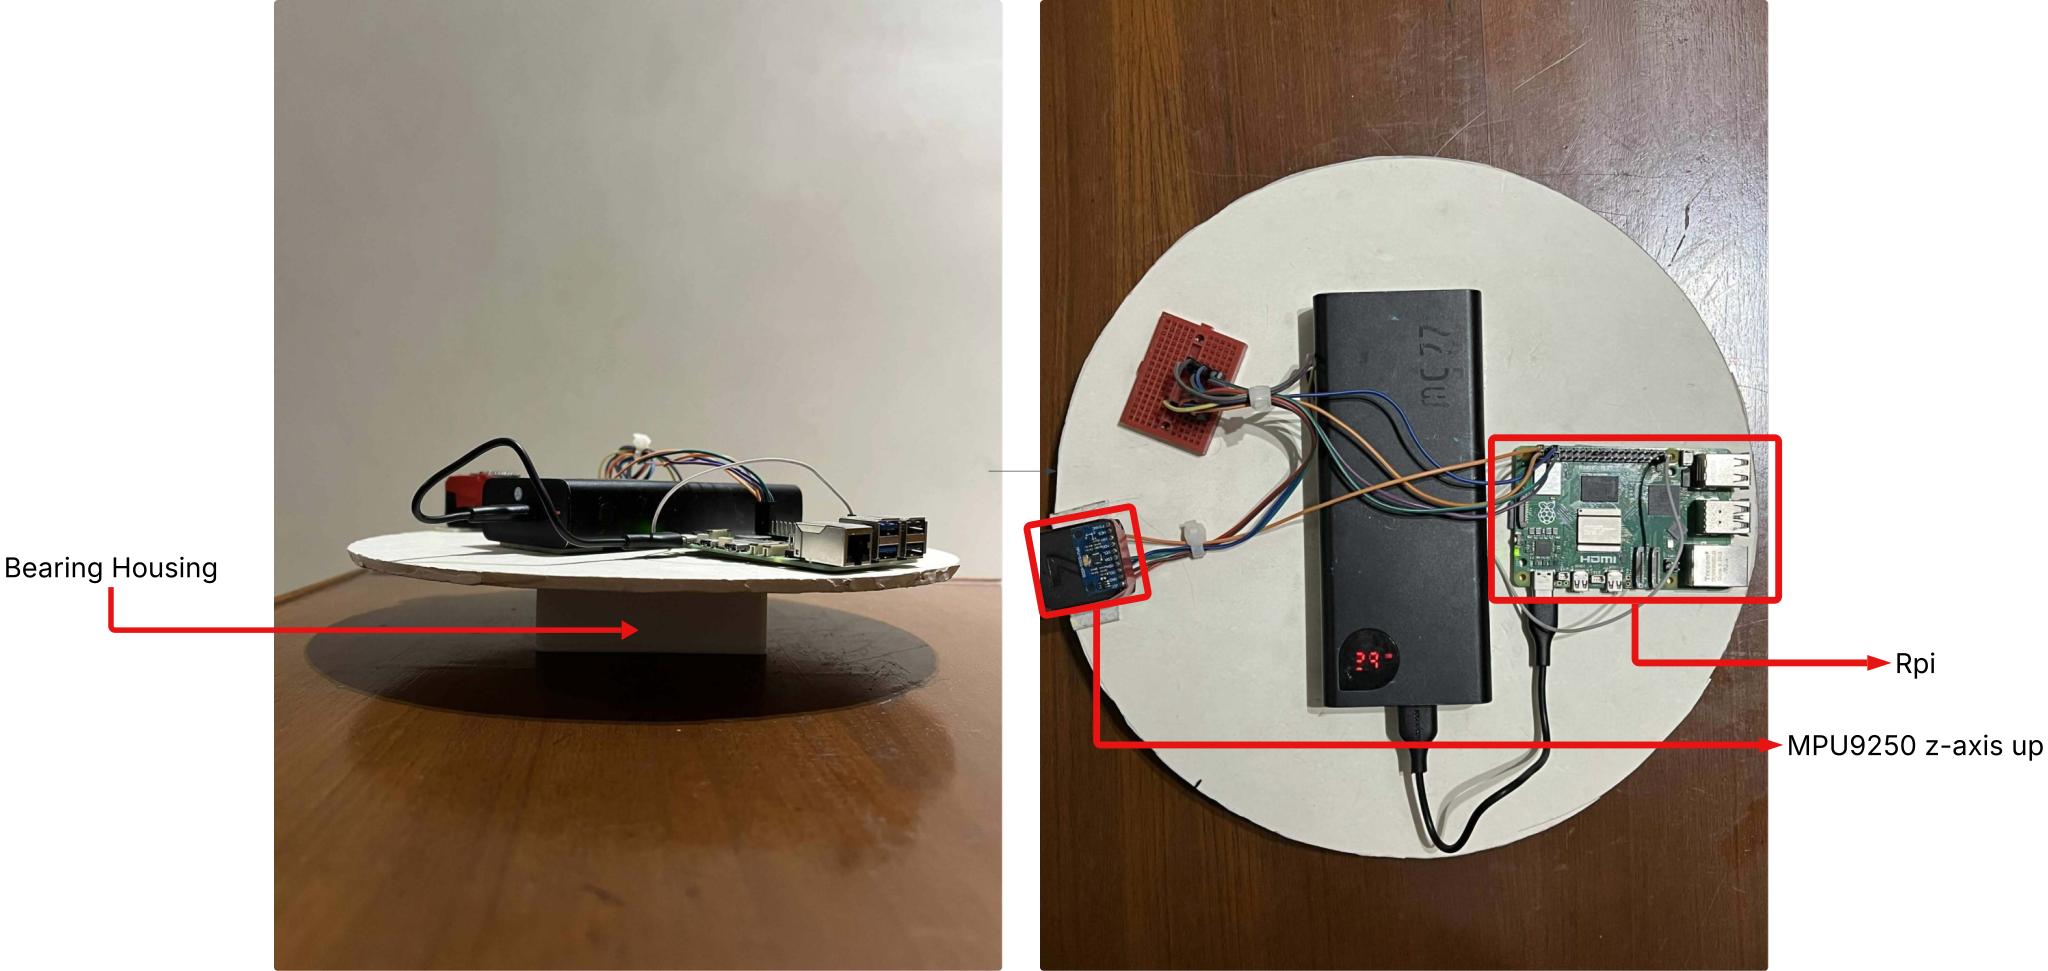
\includegraphics[width=.85\linewidth]{logos/turntable_marked.png}  
    \caption{Mechanical Turntable side view (left) and top view (right).}    
    \label{fig:turntable}
  \end{figure}
  \end{frame}
  
  
  % Frame 2: Motion Protocols & Software
  \begin{frame}{Motion Protocols \& Software Setup}
  \begin{itemize}
      \item \textbf{Motion Protocols:}
      \begin{itemize}
          \item \textbf{Static:} No movement; tests sensor stability and drift.  
          \item \textbf{Quasi-static:} Slow $0^{\circ}\!\!-\!180^{\circ}$ rotation (clockwise \& counterclockwise), two cycles per axis.  
          \item \textbf{Dynamic:} Continuous rapid rotations (3, 4, 5 turns per cycle).
      \end{itemize}
  
      \item \textbf{Software Infrastructure:}  
      \begin{itemize}
          \item Raspberry Pi runs 4 parallel Python scripts: Proposed Filter, AQUA, EKF, Madgwick.  
          \item Reads MPU9250 sensor (accel, gyro, mag) via I2C.  
          \item AS5600 encoder provides ground-truth quaternions.  
          \item All filter outputs + ground truth logged into CSV for post-processing.
      \end{itemize}
  
      \item \textbf{Result Generation:}  
      Quaternion absolute distance metric (Sec. 9.2) computed and plotted to compare filter performance under each motion type.
  \end{itemize}
  \end{frame}

  \begin{frame}{Evaluation Methodology}
    \scriptsize
    \begin{columns}[T]
      % Left column: Data & Protocol
      \begin{column}{0.48\textwidth}
        \textbf{Algorithms Under Test}
        \begin{itemize}
          \item Extended Kalman Filter (EKF)
          \item Madgwick Filter
          \item Proposed Modified Complementary Filter
          \item Algebraic Quaternion Update Algorithm (AQUA)
        \end{itemize}
      \end{column}
    
      % Right column: Metrics & Goals
      \begin{column}{0.48\textwidth}
        \textbf{Comparison Metrics}
        \begin{itemize}
          \item \textbf{Accuracy:} Quaternion absolute distance between the estimated and ground truth quaternions.
          \item \textbf{Efficiency:}
            \begin{itemize}
              \item Execution time per sample.
              \item Memory footprint.
            \end{itemize}
          \item \textbf{Robustness:}
            \begin{itemize}
              \item Static vs.\ dynamic motions.
              \item Undisturbed vs.\ disturbed conditions.
            \end{itemize}
        \end{itemize}
        \vspace{0.5em}
      \end{column}
    \end{columns}
    \end{frame}
  


\section{Results}

\begin{frame}{Results of $\alpha$-toggling and noise removal across cv_set}
\small
The charts only compare the results on 5 files of the cv\_set containing [8, 14, 17, 22, 30], as the other files were used to train the noise removal model.
\begin{table}[H]
\centering
\caption{Mean Error Statistics across the \texttt{cv\_set}}
\label{tab:error_statistics_cvset_mean}
    \begin{tabular}{|p{0.3\textwidth}|p{0.2\textwidth}|p{0.2\textwidth}|p{0.2\textwidth}|}
    \hline
    \textbf{Filename} & \textbf{Basic CF} & \textbf{Proposed CF} & \textbf{ MadgWick Filter} \\
    \hline
    09 undisturbed fast rotation with breaks B.hdf5 & 0.8134 & 0.7408 & 0.7899 \\
    \hline
    15 undisturbed fast translation A.hdf5 & 3.1007 & 1.6212 & 5.9503 \\
    \hline
    18 undisturbed fast translation with breaks B.hdf5 & 5.5009 & 1.2757 & 1.1728 \\
    \hline
    23 undisturbed fast combined 360s.hdf5 & 3.6085 & 2.7388 & 5.3682 \\
    \hline
    31 disturbed stationary magnet D.hdf5 & 2.4708 & 1.5798 & 0.6953 \\
    \hline
    \end{tabular}
\end{table}
    
\end{frame}

\begin{frame}{Results of $\alpha$-toggling and noise removal across individual files}
\small
\textcolor{red}{Red - Madgwick Filter} | \textcolor{green}{Green - Complementary Filter} | \textcolor{blue}{Blue - Our Proposed Filter} \\ 
\textbf{X-axis:} iterations \\ \textbf{Y-axis:} mean error(lower the better)

\begin{figure}
    \centering
    \includegraphics[width=1\linewidth]{logos/9_undisturbed_fast_rotation_with_breaks_B.png}
    \caption{9\_undisturbed\_fast\_rotation\_with\_breaks\_B}
    \label{fig:9_undisturbed_fast_rotation}
\end{figure}
\hfill
\end{frame}

\begin{frame}{Results of $\alpha$-toggling and noise removal across individual files}
\small
\textcolor{red}{Red - Madgwick Filter} | \textcolor{green}{Green - Complementary Filter} | \textcolor{blue}{Blue - Our Proposed Filter} \\ 
\textbf{X-axis:} iterations \\ \textbf{Y-axis:} mean error(lower the better)

\begin{figure}
    \centering
    \includegraphics[width=1\linewidth]{logos/15_undisturbed_fast_translation_A.png}
    \caption{15\_undisturbed\_fast\_translation\_A}
    \label{fig:15_undisturbed_fast_translation}
\end{figure}
\hfill
\end{frame}

\begin{frame}{Results of $\alpha$-toggling and noise removal across individual files}
\small
\textcolor{red}{Red - Madgwick Filter} | \textcolor{green}{Green - Complementary Filter} | \textcolor{blue}{Blue - Our Proposed Filter} \\ 
\textbf{X-axis:} iterations \\ \textbf{Y-axis:} mean error(lower the better)

\begin{figure}
    \centering
    \includegraphics[width=1\linewidth]{logos/18_undisturbed_fast_translation_with_breaks_B.png}
    \caption{18\_undisturbed\_fast\_translation\_with\_breaks\_B}
    \label{fig:18_undisturbed_fast_trans}
\end{figure}
\hfill
\end{frame}

\begin{frame}{Results of $\alpha$-toggling and noise removal across individual files}
\small
\textcolor{red}{Red - Madgwick Filter} | \textcolor{green}{Green - Complementary Filter} | \textcolor{blue}{Blue - Our Proposed Filter} \\ 
\textbf{X-axis:} iterations \\ \textbf{Y-axis:} mean error(lower the better)

\begin{figure}
    \centering
    \includegraphics[width=1\linewidth]{logos/23_undisturbed_fast_combined_360s.png}
    \caption{23\_undisturbed\_fast\_combined\_360s}
    \label{fig:23_undisturbed360}
\end{figure}
\hfill
\end{frame}

\section{Shortcomings}

\begin{frame}{Shortcomings of Our Data‐Driven CF}
\begin{itemize}
  \item \textbf{Model Size \& Memory:}
    XGBoost inference is $O(\log n)$ per tree (depth=15, 6 vars, 15 estimators) → wide trees consume significant memory.
  \item \textbf{Computational Overhead:}
    \begin{itemize}
      \item Matrix exponentiation for $R_g$ rotations.
      \item RANSAC‐based training adds extra latency.
    \end{itemize}
  \item \textbf{Training Time:}
    RANSAC loop and ensemble fitting are time‐intensive.
  \item \textbf{Generalizability:}
    Noticeable drop in performance on cross‐validation vs.\ test sets.
\end{itemize}
\end{frame}


\section{Future Works}




\begin{frame}{Deployment Challenges \& Strategy}
\begin{columns}[T]
  % Left column: Challenge
  \begin{column}{0.48\textwidth}
    \begin{block}{{\textbf{Challenge: Resource Constraints}}}
      \begin{itemize}
        \item XGBoost model size: 25 MB flash memory  
        \item ESP32 max flash: 4 MB  
        \item Limited CPU and RAM on embedded platforms  
      \end{itemize}
    \end{block}
  \end{column}
  
  % Right column: Solution
  \begin{column}{0.48\textwidth}
    \begin{exampleblock}{{\textbf{Proposed Strategy}}}
      \begin{itemize}
        \item \textbf{Model Optimization:}  
          \begin{itemize}
            \item Quantization \& pruning  
            \item Tree depth reduction  
            \item Converter to light-weight formats (e.g., Treelite)
          \end{itemize}
        \item \textbf{Fallback Deployment:}  
          \begin{itemize}
            \item If ESP32 still infeasible, deploy on Raspberry Pi  
            \item Leverage its higher memory and CPU capabilities  
          \end{itemize}
      \end{itemize}
    \end{exampleblock}
  \end{column}
\end{columns}
\end{frame} 

% Sample bibliography (not shown in presentation, just for reference)
\section{References}
\begin{frame}[allowframebreaks]{References}
    \small
    \printbibliography
\end{frame}


\begin{frame}[plain]
  \centering
  \Huge \textbf{Thank you!}
\end{frame}

\end{document}